\documentclass[12pt,a4paper,oneside]{article} %% Dokumenten Parameter und Art des Dokuments
\usepackage[utf8x]{inputenc} %% Diese Datei ist im utf8 Format dies ist hier damit Latex uns versteht
\usepackage[ngerman]{babel} %% Rechtschreib prüfung
\usepackage{hyperref}
\usepackage{amsmath} %% Packet zur verwendung Mathematischer Formeln
\usepackage{amsfonts}
\usepackage{amssymb} %% Packet zur verwendung Mathematischer Symbole
\usepackage{mathtools}
\usepackage{microtype} %% Sorgt für besseren umgang mit zu lange/kurzen Zeilen
\usepackage{pdfpages} %% Zum einfügen eines PDf dokuments
\title{TGI Serie 9}
\author{Bennet Bleßmann, Sven Korfmann}

\begin{document}
\maketitle

\section*{H1}

\section*{H2}


\section*{H3}

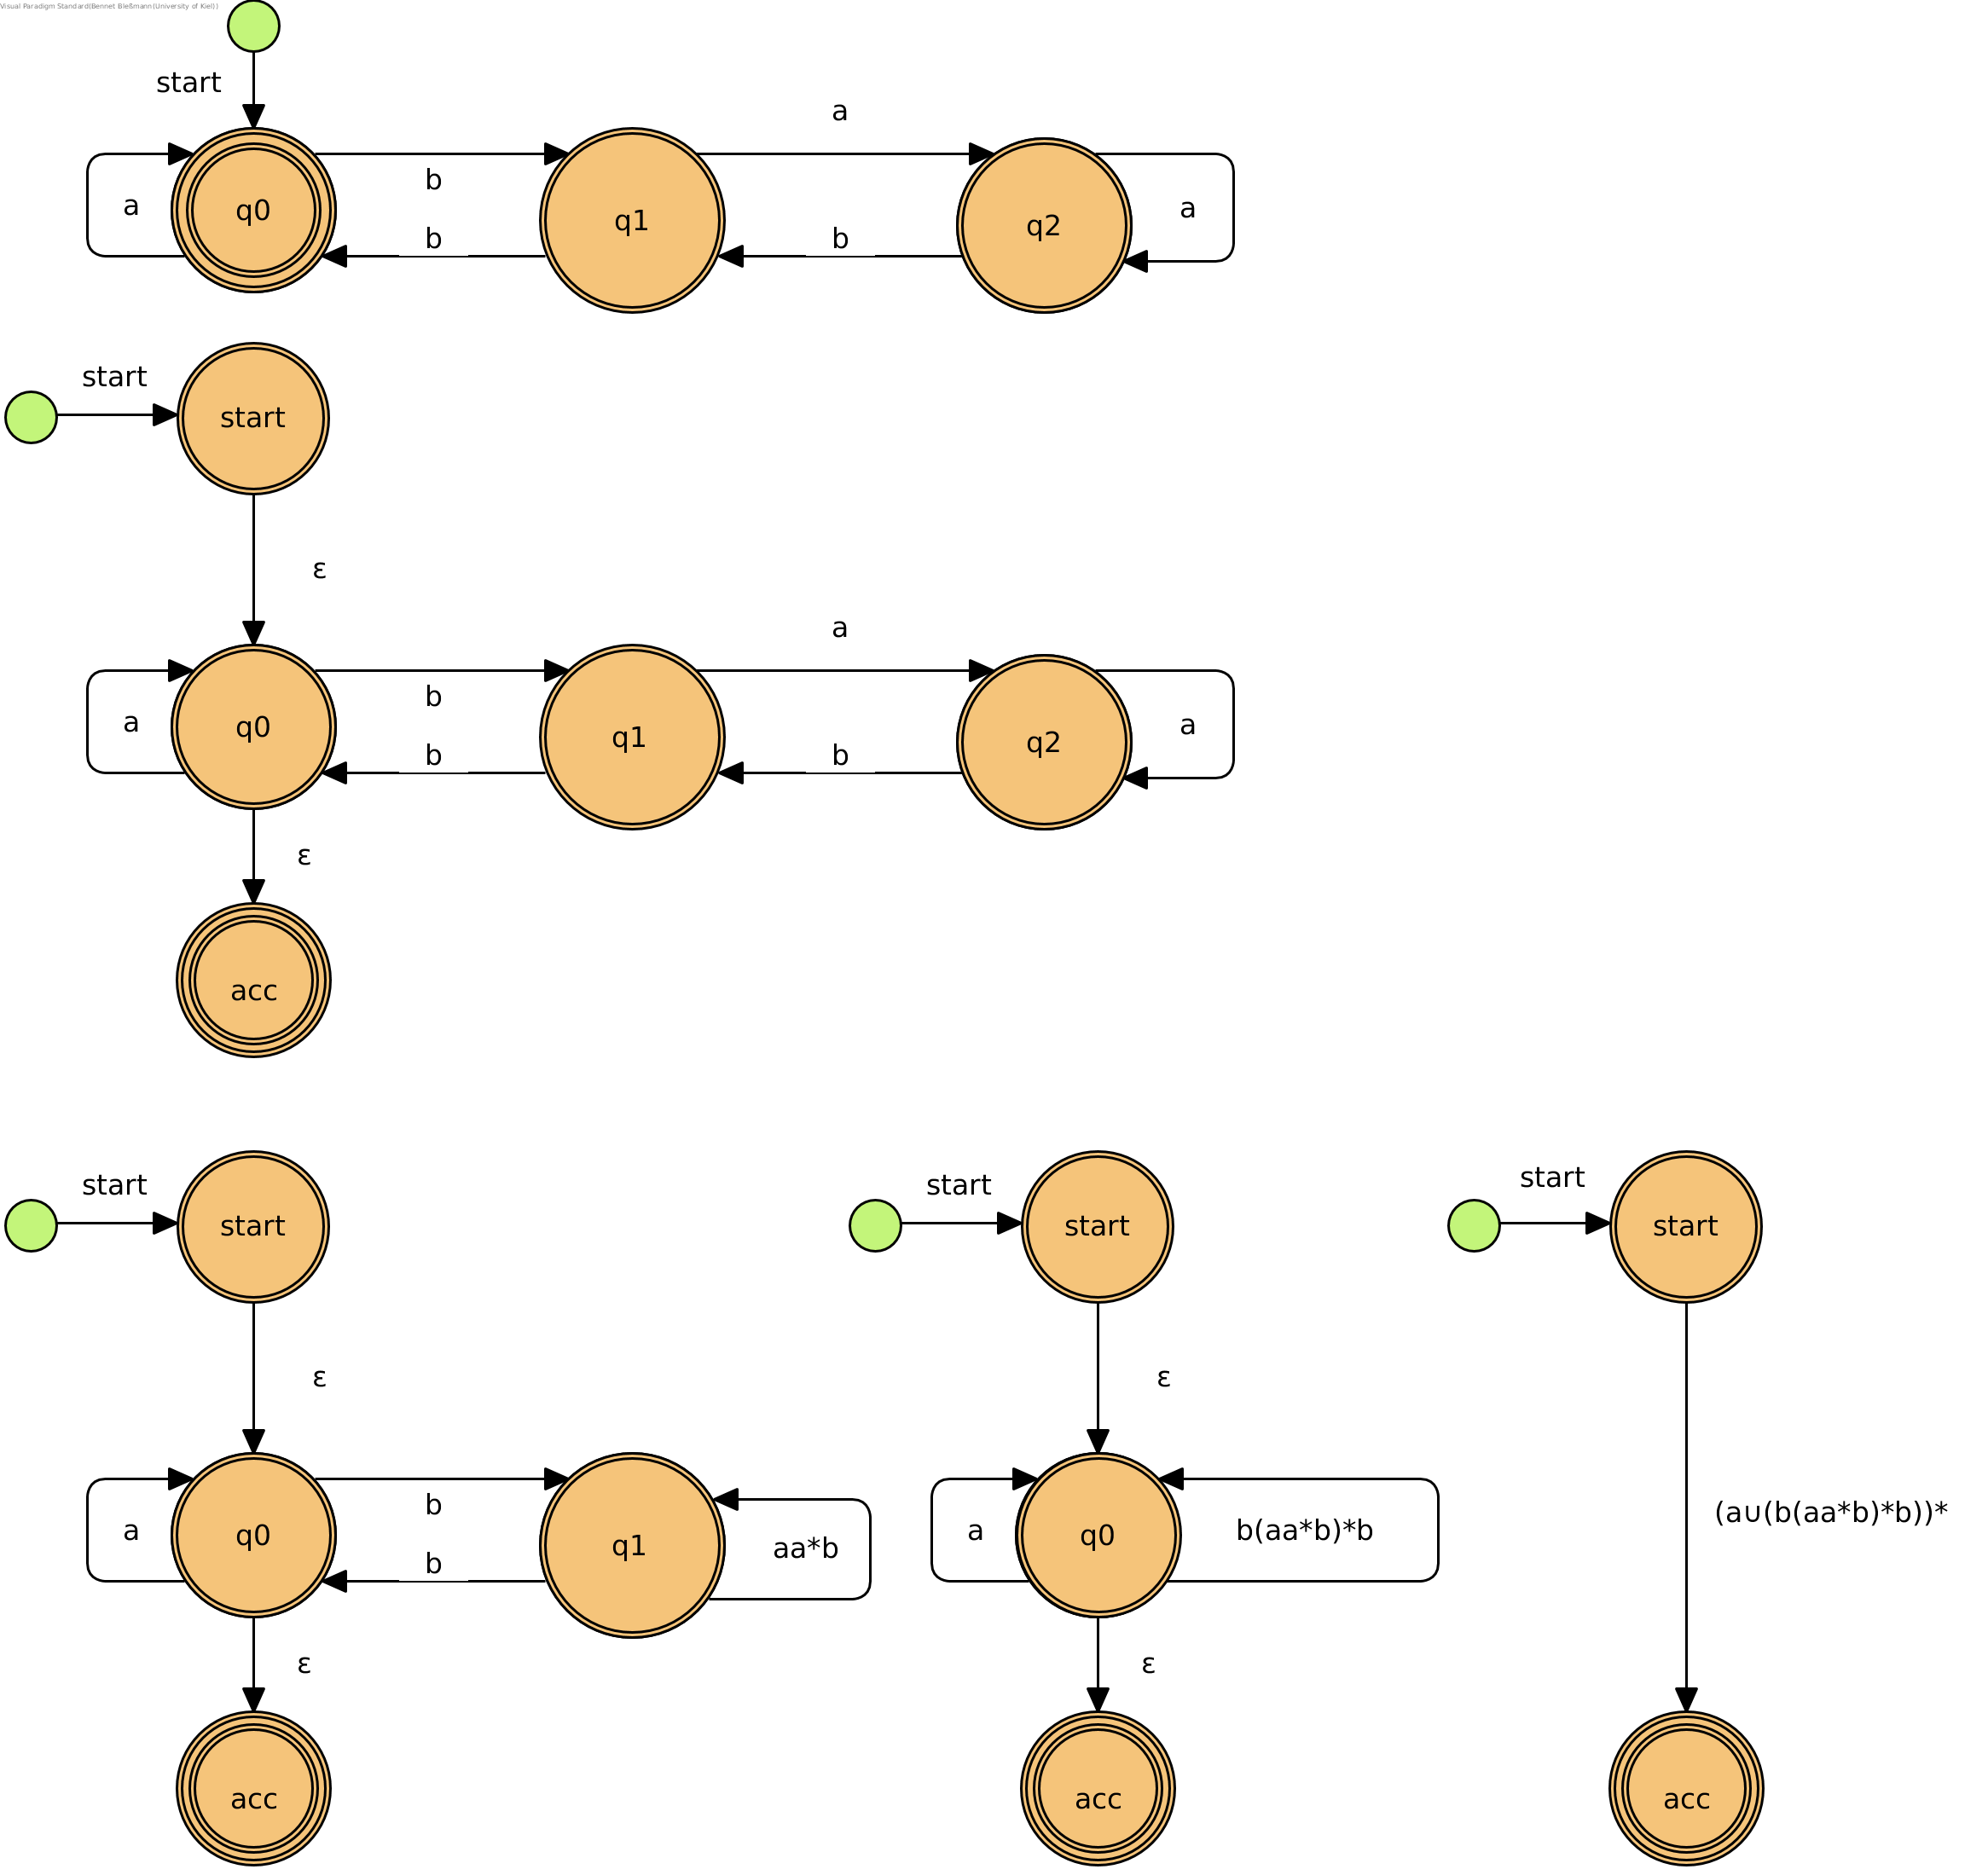
\includegraphics[width=\textwidth]{part/S9-A3.png}

$R = (a\cup(b(aa^*b)^*b))^*$



\section*{H4}

Sei $A=(Q,\Sigma,\delta,q_0,F)$ ein deterministischer endlicher Automat.

\subsection*{a)}

	\subsubsection*{Behauptung}
	
	Es gilt $\forall q \in Q, u, v \in \Sigma^*: \hat{\delta}(q,uv) = \hat{\delta}(\hat{\delta}(q,u),v)$.

	\subsubsection*{Induktion}
	Induktion über die Länge des Präfixes.

	\subsubsection*{IA}
		Es gilt für den leeren Präfix $\varepsilon$.
		
		$\forall q \in Q, u = \varepsilon, \forall v \in \Sigma^*$ gilt $\hat{\delta}(q,uv) =  \hat{\delta}(q,v) = \hat{\delta}(\hat{\delta}(q,u),v)$ 

	\subsubsection*{IV}
	Wir setzten vorraus das es für einen Präfix u gilt.
	
	Sei $u \in \Sigma^*$
	
	Und es gilt 	
	$\forall q \in Q, v \in \Sigma^*:\hat{\delta}(q,uv) =  \hat{\delta}(\hat{\delta}(q,u),v)$ 
	
	\subsubsection*{IS}
	Erweiterung des Präfixes $u$ um ein beliebiges Zeichen $a$.
	
	Sei $a \in \Sigma$.
	
	$\hat{\delta}(q,auv)
	= \hat{\delta}(\delta(q,a),uv)
	= \hat{\delta}(\hat{\delta}(\delta(q,a),u),v)
	= \hat{\delta}(\hat{\delta}(q,au),v)$
	\paragraph*{}
	Damit ist die Behauptung gezeigt.
	  
	  \newpage
\subsection*{b)}

\subsubsection*{Behauptung}
$L(A_{\text{präfix}}) = \text{PRÄFIX}_{L(A)}$

\subsubsection*{Beweis}

$L(A_{\text{präfix}})$
$ = \{z \in \Sigma^* | \hat{\delta}(q_0,z) \in \{q \in Q| \exists w \in \Sigma^* : \hat{\delta}(q,w)\in F\}\}$

$ = \{z \in \Sigma^* | \exists w \in \Sigma^* : \hat{\delta}(\hat{\delta}(q_0,z),w)\in F\}$


$ = \{z \in \Sigma^* | \exists w \in \Sigma^* : \hat{\delta}(q_0,zw)\in F\}$


$ = \{z \in \Sigma^* | \exists w \in \Sigma^* : zw \in L(A)\}$

$ = \text{PRÄFIX}_{L(A)}$


\subsection*{c)}

Aus einem DEA $A$ der eine Sprache entscheidet, lässt sich ein DEA $A_{\text{präfix}}$ konstruieren der alle Präfixe der Sprache erkennt indem nur die akzeptierenden Zustände geändert werden,
so dass genau die Zustände $q$ in $A_{\text{präfix}}$ akzeptieren, zu denen ein Wort existiert welches in $A$ von $q$ in einen akzeptierenden Zustand führt.

Der so entstehende Automat akzeptiert dann alle Worte zu denen ein Suffix existiert, so dass das Wort konkateniert mit dem Suffix ein gültiges Wort im original Automaten ist.
Ein solches Wort ist also ein Präfix.

%\include{part/S9-A5}
	
\end{document}